\documentclass[11pt,a4paper]{article}
\usepackage[T1]{fontenc}
\usepackage[utf8]{inputenc}
\usepackage{lmodern}
\usepackage[margin=2.5cm]{geometry}
\usepackage{amsmath,amssymb}
\usepackage{booktabs}
\usepackage{graphicx}
\usepackage[hidelinks]{hyperref}
\hypersetup{pdfauthor={Gianni Pilotti},pdftitle={Equity Valuation: DCF and Comparables},pdfcreator={},pdfproducer={}}
\setlength{\parindent}{0pt}
\setlength{\parskip}{6pt}

\title{Equity Valuation: DCF and Comparables}
\author{Gianni Pilotti}
\date{}

\begin{document}
\maketitle

\section{The Core Idea}

A stock price is a claim on future cash flows. A valuation model turns assumptions about those cash flows and the discount rate into a value per share, which can be compared with the market price. The toolkit does this for 10 large US stocks with two standard methods and checks how much the answer depends on its inputs.

\begin{itemize}
\item \textbf{DCF:} project free cash flow, discount it at the WACC, add a terminal value.
\item \textbf{Comparables:} apply the median EV/EBITDA multiple of the group to each company's EBITDA.
\end{itemize}

The results show the limits of the methods as much as they show mispricing. A gap of $-90\%$ points to a mismatch between the model and the company, not to a trading signal.

\section{Method}

\subsection{Cost of Capital}

The code (\texttt{equity\_valuation.py}) uses a risk-free rate of 4\%, a market risk premium of 5\%, a flat cost of debt of 5\% and a tax rate of 21\%. With the Yahoo Finance beta $\beta$:
\begin{equation}
k_e=r_f+\beta\cdot\text{MRP},\qquad
\text{WACC}=\frac{E}{E+D}\,k_e+\frac{D}{E+D}\,k_d(1-t).
\end{equation}
$E$ is the market capitalisation and $D$ the total debt.

\subsection{DCF}

The starting free cash flow $F_0$ comes from Yahoo Finance. The growth rate fades linearly over 5 years from the reported revenue growth $g_1$ (clipped to $[-5\%,\,20\%]$) to the terminal growth $g=2.5\%$:
\begin{equation}
g_t=g_1+\frac{t-1}{4}\,(g-g_1),\qquad F_t=F_{t-1}(1+g_t),\quad t=1,\dots,5.
\end{equation}
Cash flows are discounted at year end. The Gordon terminal value and the equity value are
\begin{equation}
TV=\frac{F_5(1+g)}{\text{WACC}-g},\qquad
EV=\sum_{t=1}^{5}\frac{F_t}{(1+\text{WACC})^t}+\frac{TV}{(1+\text{WACC})^5},
\end{equation}
\begin{equation}
\text{Value per share}=\frac{EV-(\text{debt}-\text{cash})}{\text{shares outstanding}}.
\end{equation}
The model returns no value when $F_0\le0$ or missing.

\subsection{Comparables}

The implied price of each stock is
\begin{equation}
P^{\text{comps}}=\frac{m^{\ast}\cdot\text{EBITDA}-\text{net debt}}{\text{shares}},
\end{equation}
where $m^{\ast}$ is the median of EV/EBITDA over the group.

\subsection{Sensitivity}

For the largest stock by market capitalisation (NVDA), the DCF is recomputed on a grid of 5 WACC values (base $\pm2$ points) and 5 terminal growth values (2.5\% $\pm1$ point). Cells with WACC $\le g$ are left empty.

\section{Results}

Valuation screen from \texttt{output/valuation\_screen.csv}. Prices are in dollars as downloaded.

\begin{center}
\begin{tabular}{lrrrrrr}
\toprule
Ticker & Price & WACC & DCF value & DCF upside & Comps value & Comps upside \\
\midrule
XOM   & 153.04 & 4.8\%  & 320.69 & $+109.5\%$ & 310.01 & $+102.6\%$ \\
UNH   & 407.08 & 6.6\%  & 545.97 & $+34.1\%$  & 471.69 & $+15.9\%$ \\
PG    & 145.79 & 5.7\%  & 167.40 & $+14.8\%$  & 195.25 & $+33.9\%$ \\
JNJ   & 259.24 & 5.1\%  & 296.25 & $+14.3\%$  & 268.73 & $+3.7\%$ \\
AAPL  & 313.33 & 9.3\%  & 148.66 & $-52.6\%$  & 221.55 & $-29.3\%$ \\
KO    & 87.05  & 5.5\%  & 38.87  & $-55.3\%$  & 70.09  & $-19.5\%$ \\
GOOGL & 354.30 & 10.0\% & 97.54  & $-72.5\%$  & 592.78 & $+67.3\%$ \\
NVDA  & 223.96 & 15.0\% & 24.12  & $-89.2\%$  & 134.11 & $-40.1\%$ \\
MSFT  & 499.99 & 9.3\%  & 39.73  & $-92.1\%$  & 499.99 & $0.0\%$ \\
\bottomrule
\end{tabular}
\end{center}

\begin{itemize}
\item \textbf{Growth stocks:} NVDA, MSFT, GOOGL and AAPL come out far below the market price. A 5-year fade to 2.5\% growth cannot reproduce the growth the market expects.
\item \textbf{Low WACC:} XOM has a WACC of 4.8\%, only 2.3 points above the terminal growth rate. This inflates the terminal value and the upside.
\item \textbf{MSFT in comps:} its upside is zero by construction, since its own multiple is the group median.
\item \textbf{JPM:} no value. Yahoo Finance gives no usable free cash flow or EBITDA for a bank, and the methods do not suit banks.
\end{itemize}

NVDA sensitivity (\texttt{output/sensitivity\_NVDA.csv}): the value per share runs from \$19.9 (WACC 17\%, $g=1.5\%$) to \$31.0 (WACC 13\%, $g=3.5\%$). Both ends are far below the price of \$223.96.

\begin{figure}[ht]
\centering
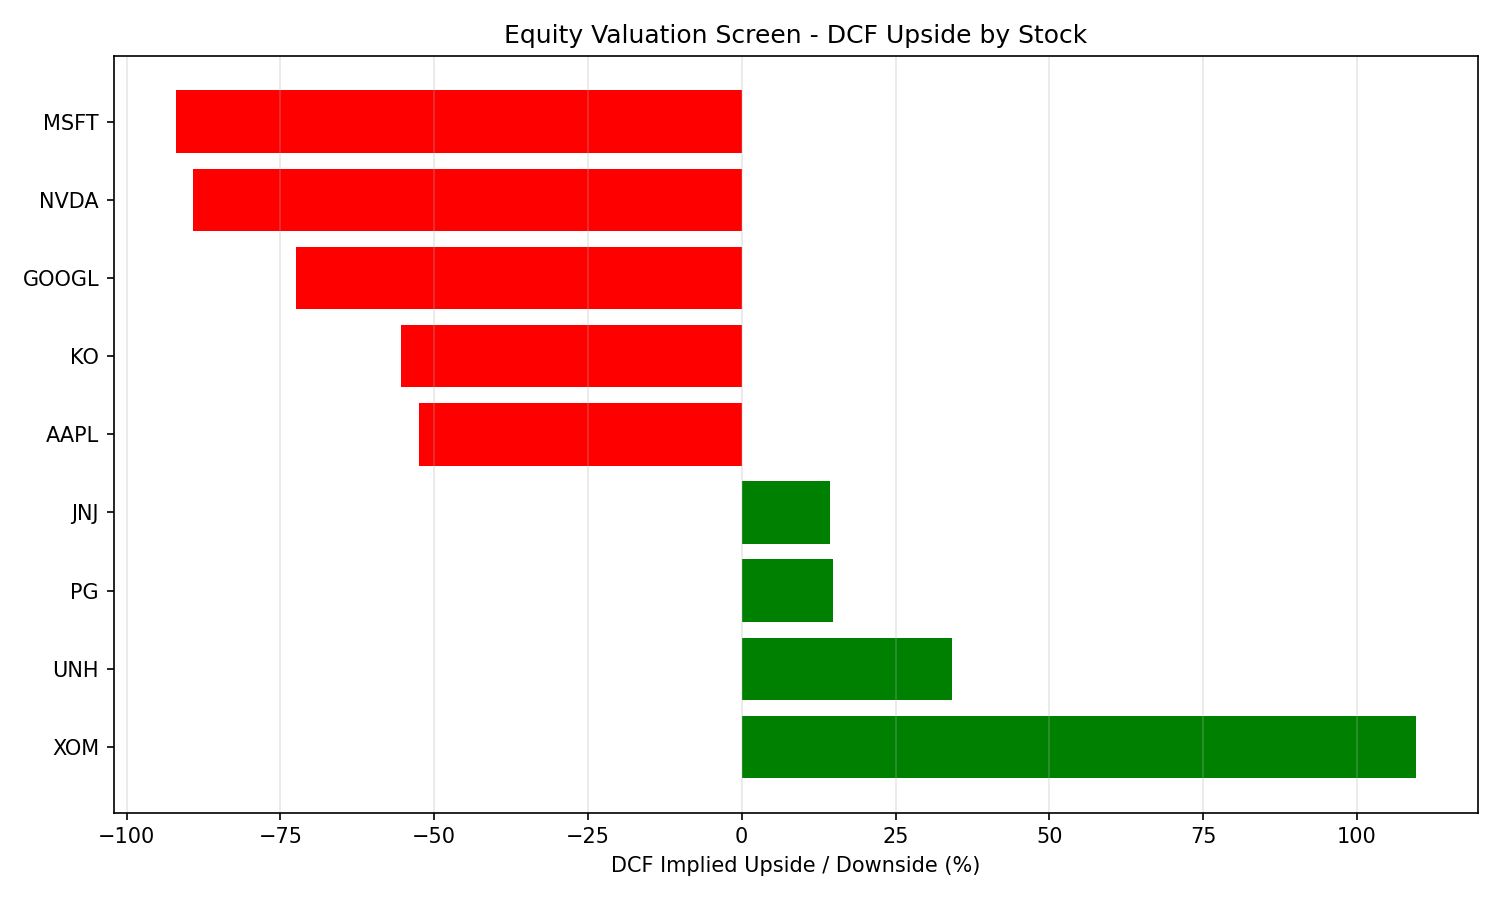
\includegraphics[width=0.8\textwidth]{../output/valuation_screen.png}
\caption{DCF implied upside or downside by stock.}
\end{figure}

\section{Worked Example}

The inputs are illustrative: $F_0=100$, $g_1=10\%$, beta 1.2, market cap 800, debt 200, cash 50, 10 shares.

\textbf{WACC.} $k_e=4\%+1.2\cdot5\%=10\%$. Weights are $800/1000=0.8$ and $0.2$. $\text{WACC}=0.8\cdot10\%+0.2\cdot5\%\cdot(1-0.21)=8.79\%$.

\textbf{Cash flows.} The growth path is $10\%,\,8.125\%,\,6.25\%,\,4.375\%,\,2.5\%$, which gives $F_{1..5}=110.00,\,118.94,\,126.37,\,131.90,\,135.20$.

\textbf{Present value.} The discount factors $1.0879^{-t}$ are $0.9192,\,0.8449,\,0.7767,\,0.7139,\,0.6562$, so $\sum F_t\,DF_t=482.64$.

\textbf{Terminal value.} $TV=135.20\cdot1.025/(0.0879-0.025)=2203.14$. Its present value is $2203.14\cdot0.6562=1445.76$.

\textbf{Equity value.} $EV=482.64+1445.76=1928.40$. Net debt is $200-50=150$. Value per share $=(1928.40-150)/10=177.84$.

The terminal value is 75.0\% of $EV$. Moving the WACC by 2 points changes the value per share to 268.57 (WACC 6.79\%) or 130.91 (WACC 10.79\%).

\textbf{Comps.} With an illustrative median multiple of $12\times$ and EBITDA of 200, the implied price is $(12\cdot200-150)/10=225$.

\section{Limits}

\begin{itemize}
\item \textbf{Terminal value dominates:} in the example it is three quarters of the value, so the result rests on WACC and $g$.
\item \textbf{Flat assumptions:} one risk-free rate, one risk premium and one cost of debt for all companies. A low beta pushes the WACC toward $g$ and inflates the terminal value.
\item \textbf{Raw data:} Yahoo Finance fundamentals are not adjusted. There are no analyst estimates and no removal of one-off items.
\item \textbf{Small peer group:} the median multiple comes from 9 companies of different sectors, so it mixes unlike businesses.
\item \textbf{Banks excluded:} the methods do not apply to JPM.
\end{itemize}

\end{document}
